\section{\textit{Cost-Sensitive Classification} (Bonus)}
\label{sec:cost-sensitive}

Pada persoalan ini, kelas positif adalah pemesanan yang batal. \textit{False positive} berarti
pemesanan diprediksi batal padahal tamunya datang. Jika penginapan menjual ulang kamar tersebut,
penginapan menjadi \textit{overbooked}. \textit{False negative} berarti pembatalan tidak terdeteksi,
sehingga kamar kosong tanpa disiapkan penggantinya. Spesifikasi menetapkan bahwa \textit{false
positive} dua kali lebih mahal daripada \textit{false negative} (Tabel~\ref{tab:cost-matrix}).

\begin{table}[H]
	\centering
	\caption{Matriks biaya (kelas positif = batal)}
	\label{tab:cost-matrix}
	\begin{tabular}{l c c}
		\toprule
		& \textbf{Prediksi: tidak batal} & \textbf{Prediksi: batal} \\
		\midrule
		\textbf{Aktual: tidak batal} & 0 & $C_{FP} = 2$ \\
		\textbf{Aktual: batal} & $C_{FN} = 1$ & 0 \\
		\bottomrule
	\end{tabular}
\end{table}

\subsection{Pendekatan}

Pendekatan ini diterapkan pada model DTL final (Subbab~\ref{sec:dtl}). Total biaya untuk sebuah
prediksi adalah
\begin{equation}
	\text{Biaya} = C_{FP} \cdot FP + C_{FN} \cdot FN = 2\,FP + FN.
\end{equation}
Dua cara penanganan dibandingkan dengan skema standar.
\begin{enumerate}
	\item \textbf{\textit{Threshold moving}.} Model tidak dilatih ulang. Jika peluang daun
	terkalibrasi, keputusan dengan biaya harapan terkecil adalah menyatakan batal ketika
	$P(\text{batal} \mid x) \ge C_{FP} / (C_{FP} + C_{FN}) = 2/3$ \cite{elkan2001cost}.
	\item \textbf{Pembobotan kelas.} Contoh kelas tidak batal diberi bobot 2 saat pelatihan
	(\texttt{class\_weight=\{0: 2, 1: 1\}}), lalu dipakai \textit{threshold} 0,5. Bobot ini masuk ke
	perhitungan entropi, pemilihan pemecahan, dan \textit{pruning}, sehingga bentuk pohon ikut berubah
	\cite{ting2002instance}.
\end{enumerate}
Semua skema dievaluasi pada prediksi \textit{out-of-fold} dari validasi silang 5-\textit{fold} yang
sama dengan Subbab~\ref{subsec:dtl-validasi} (\textit{seed} 42). Data latih berisi 27.309 baris dengan
8.944 pemesanan batal.

\subsection{Hasil dan Analisis}

\begin{table}[H]
	\centering
	\caption{Perbandingan skema standar dan \textit{cost-sensitive} pada DTL (prediksi OOF, \textit{seed} 42)}
	\label{tab:cost-hasil}
	\begin{tabular}{l c c c c}
		\toprule
		\textbf{Skema} & \textbf{FP} & \textbf{FN} & \textbf{Total biaya} & \textbf{Macro F1} \\
		\midrule
		Standar, \textit{threshold} 0,4 (submisi Kaggle) & 1.210 & 1.875 & 4.295 & 0,8692 \\
		Standar, \textit{threshold} 0,5 & 1.202 & 1.882 & 4.286 & 0,8692 \\
		\textit{Threshold moving}, $2/3$ & 1.141 & 1.971 & 4.253 & 0,8674 \\
		Pembobotan kelas 2 : 1, \textit{threshold} 0,5 & 817 & 2.490 & \textbf{4.124} & 0,8550 \\
		\bottomrule
	\end{tabular}
\end{table}

\begin{figure}[H]
	\centering
	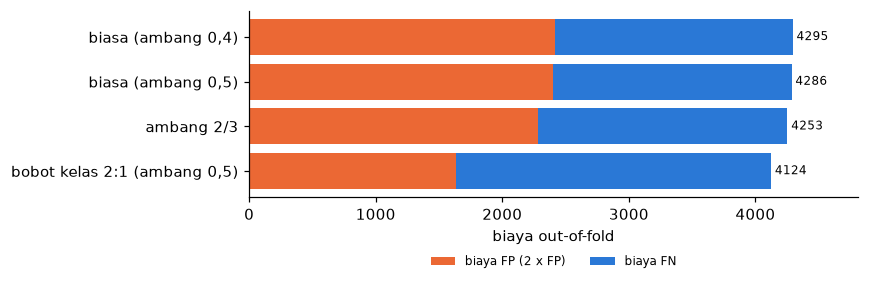
\includegraphics[width=0.85\textwidth]{dtl/dtl_cost_sensitive.png}
	\caption{Komposisi total biaya OOF setiap skema: biaya FP ($2 \times FP$) dan biaya FN}
	\label{fig:cost-sensitive}
\end{figure}

\paragraph{\textit{Threshold moving} hampir tidak berpengaruh.} Menggeser \textit{threshold} dari 0,5
ke $2/3$ hanya menurunkan biaya dari 4.286 menjadi 4.253 (0,8\%). Sebanyak 61 \textit{false positive}
hilang dan 89 \textit{false negative} bertambah. Pohon final memiliki daun yang sangat murni, sehingga
hanya sedikit pemesanan yang peluangnya berada di antara 0,5 dan $2/3$. Akibatnya, menggeser
\textit{threshold} di rentang ini hanya mengubah sebagian kecil prediksi.

\paragraph{Pembobotan kelas lebih efektif.} Dengan bobot 2 : 1, \textit{false positive} turun dari
1.202 menjadi 817, dengan tambahan 608 \textit{false negative}, dan total biaya turun menjadi 4.124.
Dibandingkan skema standar dengan \textit{threshold} 0,5, penurunannya 162 (3,8\%), hampir lima kali
penurunan dari \textit{threshold moving}. Pembobotan bekerja saat pelatihan, sehingga pohon membuat
pemecahan dan daun baru, bukan hanya menggeser keputusan pada daun yang sama. Harganya adalah Macro F1
yang turun 0,0142, karena Macro F1 tidak membedakan biaya kedua jenis kesalahan.

\paragraph{Keterbatasan.} Semua angka berasal dari satu \textit{seed} pembagian, dan bobot kelas hanya
diuji pada satu nilai (2 : 1, sesuai matriks biaya). Selisih biaya antara skema standar dan
\textit{threshold moving} (33) kecil, sehingga dapat berubah pada \textit{seed} lain.

Kedua tujuan memerlukan model yang berbeda. Submisi Kaggle tetap memakai model standar dengan
\textit{threshold} 0,4 karena kompetisi dinilai dengan Macro F1. Untuk penginapan yang memakai
prediksi ini untuk menjual ulang kamar, kami menyarankan model dengan pembobotan kelas 2 : 1, karena
model itu paling jarang salah menandai tamu yang sebenarnya datang.
